% template!!
\documentclass[sigconf,anonymous]{acmart}

\usepackage{amsmath}
\usepackage[linesnumbered,boxed]{algorithm2e}
\usepackage{subfigure}
\usepackage{graphicx}
\usepackage{color}
\usepackage{multirow}
\usepackage{colortbl}
\usepackage{tikz}
\usetikzlibrary{bayesnet}

\newenvironment{shrinkeq}[1]
{ \bgroup
  \addtolength\abovedisplayshortskip{#1}
  \addtolength\abovedisplayskip{#1}
  \addtolength\belowdisplayshortskip{#1}
  \addtolength\belowdisplayskip{#1}}
{\egroup\ignorespacesafterend}



\setcopyright{none}

\begin{document}

%???MNAR title?
\title{Drug Target Interaction Prediction with Missing not at Random Labels}

%\author{Chen Lin, Sheng Ni, Xiangxiang Zeng}
\begin{abstract}
We introduce a novel probabilistic model, \textbf{F}actorization with \textbf{M}issing \textbf{N}ot at \textbf{R}andom \textbf{L}abels (FMNRL), for \textbf{D}rug-\textbf{T}arget \textbf{I}nteraction (DTI) prediction. DTI prediction is usually modeled as a binary classification problem. Unlike previous studies which label unknown DTIs as negative samples, we treat the unknown DTIs as missing not at random labels. The proposed model, FMNRL assumes the binary DTI labels are probabilistically generated from feature vectors of both drugs and targets, and a hidden matrix mapping from the drug features to target features. By associating the possibility of a missing label with the sign of the label, FMNRL can learn the hidden feature space mapping better, and thus can provide more accurate DTI predictions. Experimental results show that FMNRL outperforms state-of-the-art methods.
\end{abstract}


\keywords{Missing Not At Random, Drug Target Interaction Prediction, Probabilistic Factor Models}

\maketitle
\section{Introduction}\label{sec:introduction}
%Background: DTI
\textbf{D}rug-\textbf{T}arget \textbf{I}nteraction (DTI) is fundamental to drug discovery and design. As biochemical experimental methods for DTI identification are extremely costly and time-consuming, computational DTI prediction methods have received a growing popularity in literature. The majority of existing computational methods treat DTI prediction as a binary classification task, where known DTIs are labeled as positive and unknown DTIs are labeled as negative~\cite{Ding2013Similarity}. To address the imbalanced problem arised from the binary classification scheme, many research has attempted to extract a subset of reliable negative samples, e.g. by random sampling~\cite{Luo2017Network} or by \textbf{P}ositive \textbf{U}nlabel \textbf{L}earning (PU Learning)~\cite{Peng2017Screening}.

%MNAR intuition
Instead of labeling the unknown DTIs as negative, we argue that it is more natural to consider the unknown DTIs, i.e. DTIS that are neither identified in vivo to be positive nor experimentally validated to be negative (non-interacting drug-target pairs), as missing labels. Furthermore, our assumption in this work is that labels are not missing at random. This is an intuitive and reasonable assumption, because researchers will use their domain expertise to filter DTIs with a high possibility to be positive and prioritize validations for these DTIs in vivo. For example, researchers find the efficacy target of a drug based on principles of biochemistry, biophysics, genetics and chemical biology. If ample evidences exist to support positive interactions with the target, then the possibility of a positive DTI is high, and the researchers are likely to conduct in vivo experiments. On the contrary, drug target interactions that are less likely to be positive are more likely to be ignored by researchers and their labels are likely to be missing.

\subsection{Contribution}
%present work
Our chief contribution in this work is a novel \textbf{F}actorization with \textbf{M}issing \textbf{N}ot at \textbf{R}andom \textbf{L}abels model (FMNRL). To the best of our knowledge, this is the first time missing not at random theory is applied in DTI identification. The inputs of FMNRL are feature vectors of drugs and targets, the partially observed labels, and the fully observed responses (i.e. labels are given or missing). The feature vectors are leant and integrated from heterogenous sources. The labels and responses are binary variables. The FMNRL model mimics the probabilitic procedures to generate labels from feature vectors and responses from labels. Specifically, the labels are related to feature vectors of both drugs and targets, and a hidden matrix mapping from the drug features to target features. The possibility of giving a response is associated with the sign of the label.

We conduct experiments on the latest DTI database. \textbf{A}rea \textbf{U}nder \textbf{R}eceiver \textbf{O}perating \textbf{C}haracteristic curve (AUROC) and \textbf{A}rea \textbf{U}nder \textbf{P}recision \textbf{R}ecall curve (AUPR) are the most commonly adopted metrics to evaluate DTI prediction performance. Our model achieves best AUPR and AUROC results on both full dataset and sample sets with balanced numbers of positive and negative labels. %Moreover, in the biomedical field, AUPR is considered to be a more robust and accurate assessment than AUROC~\cite{Luo2017Network}. Thus our significant improvment in AUPR is promising.
\subsection{Related Work}
%distinguision
One component of our work (i.e labels are generated by feature vectors learnt and fused from heterogenous information networks) is inspired by a recent work DTINet~\cite{Luo2017Network}. However, there are three key differences between our work and DTINet. (1) DTINet is based on deteministic matrix factorization, our work is based on probabilistic factor models. For example, the hidden feature space mapping matrix, labels, and responses are all random variables. This setting enables the FMNRL model to regulate the parameters (i.e. hidden feature space mapping matrix) by introducing approapriate priors. Therefore, performance on sparse dataset is improved. (2) DTINet is based on randomly missing responses, i.e. it samples uniformly a set of unknown DTIs as negative sample, while FMNRL is based on missing not at random theories. Statistical theory in~\cite{Little1987Statistical} shows that applying a model based on missing at random assumptions can lead to biased parameter estimation on data sets with missing not at random entries. (3) DTINet adopts only a subset of unknown DTIs to preserve a balanced number of positive and negative samples, while our model uses all information in the data set.

We also want to distinguish our work with another line of research. Usually only positive DTIs are deposited in known databases. Due to the lack of negative samples, PU learning has been empolyed in DTI identification, e.g. to facilitate negative sample extraction~\cite{Peng2017Screening}. PU learning does not explicitly associate the status of an instance (i.e. being labeled or unlabeled) with the value of its label. We also want to mention here that, although we experiment with datasets where only positive DTIs are deposited, FMNRL is extendable without difficulty to databases where positive and negative DTIs are available. Thus our model is applicable in more scenarios.


%structure
%This paper is structured as follows.

\section{The Proposed Method}\label{sec:method}
We start with the problem definitions and notations in Sec.~\ref{sec:input}. We then describe the proposed model FMNRL in Sec.~\ref{sec:model}. Finally we present the inference algorithm in Sec.~\ref{sec:inference}.

\subsection{Preliminaries}\label{sec:input}
DTI identification is often modeled as a binary classification task. Formally, we are given $P\in \mathcal{R}^{N\times M}$ a set of DTI labels, where $p_{i,j}=0$ indicates a negative interaction between drug $i$ and target $j$, $p_{i,j}=1$ indicates a positive DTI, the feature vectors on drug side $X\in \mathcal{R}^{N \times K}$, where $x_{i,k}$ represents drug $i$'s weight on drug feature $k$, the feature vectors on target side $Y\in \mathcal{R}^{M \times L}$, where $y_{j,l}$ represents target $j$'s weight on target feature $l$. The problem is to predict for a new drug-target pair $<i',j'>$, the possibility of a positive DTI $p(p_{i',j'}=1)$.

It is worthy to note that many previous studies have shown that extracting features $X,Y$ from heterogenous data sources are beneficial. Similar to DTINet~\cite{Luo2017Network}, we use a compact feature expression learnt from aggregating diffusion probabilities on multiple information networks. For example, on the drug side, we can collect drug side-effect network, drug similarity network and so on. On the target side, we can collect protein disease network, protein protein network and so on. The feature learning phase is beyond the scope of this paper. We refer the readers to~\cite{Luo2017Network}.

In addition to the features $X,Y$ and labels $P$, we make one essential modification to the problem definition. We assume that the inputs also contain responses $R\in \mathcal{R}^{N\times M}$, where $R_{i,j}=0$ indicates an unknown DTI, $R_{i,j}=1$ indicates a verified DTI (positive or negative). For positive responses $R_{i,j}=1$, the labels $P_{i,j}$ are observed. For negative responses $R_{i,j}=0$, the labels are hidden and unknown.

\subsection{FMNRL Model}\label{sec:model}

We use a factor model, depicted in Fig.~\ref{fig:model}. The features $X,Y$ are in different dimensions. To associate the drug features with the target features, we introduce a hidden matrix $Z\in\mathcal{R}^{K\times L}$, where $Z_{k,l}$ is a projection that maps the drug feature $k$ to the target feature $l$. We assume that $Z$ is sampled from a Gaussian distribution,

\begin{equation}\label{equ:z}
\forall k,l, Z_{k,l}\sim \mathcal{N}(0,\sigma^2),
\end{equation}
where $\sigma^2$ is the variance. We use zero mean to favor sparse feature mapping, i.e. a drug feature $k$ is associated with a few target features.

\begin{figure}
  \centering
\scalebox{0.8}{
  \tikz[yscale=0.5]{ %
%hyper parameters
  %latent nodes
    \node[const] (x) {$X$} ; %
    \node[const, right =of x] (y) {$Y$};
     \node[const, right =of y] (sigma) {$\sigma^2$};
    \node[latent, below = of sigma] (z) {$Z$};
       %per interaction
    \node[obs, below=2 of z](p){$P$};
      \node[obs, below= of p] (r){$R$};
  \node[latent, right = 2 of r] (beta){$\beta$};
  \node[const,right = of beta](eta) {$\eta$};
    \edge{x}{p};
    \edge{sigma}{z};
    \edge{y}{p};
    \edge{z}{p};
    \edge{p}{r};
  \edge{beta}{r};
  \edge{eta}{beta};
     \plate[inner sep=0.2cm, xshift=-0.12cm, yshift=0.12 cm] {plate} {(p) (r)} {N};
   \plate[inner sep=0.2cm, xshift=-0.12cm, yshift=0.12 cm] {plate2} {(beta)} {2};
 }}
\vspace*{-5pt}
\caption{Graphical Representation of the FMNRL model}\label{fig:model}
\end{figure}

We then assume that the binary label $P_{i,j}$ is generated from the following process:
\begin{equation}\label{equ:p}
\forall i,j, p(P_{i,j}=1|X,Y,Z)=\frac{1}{1+\exp{(-XZY)}_{i,j}}.
\end{equation}

The binary response is sampled from a Bernouli distribution. The parameters of the Bernouli distribution are related to the value of each $P_{i,j}$. Therefore we define $\beta_p\in\mathcal{R}^{2},p\in \{0,1\}$, $\forall p, \beta_{p,0}>0,\beta_{p,1}>0,\beta_{p,0}+\beta_{p,1}=1$, we have:
\begin{eqnarray}
\forall p\in \{0,1\}, \beta_p \sim Beta(\eta),\\
\forall i,j, R_{i,j} \sim Bern (\beta_{P_{i,j},1}),
\end{eqnarray}
where $\eta$ is the hyperparameter for the Beta distribution.

\subsection{Inference}\label{sec:inference}
The objective is to maximize the likelihood which consists of two terms. The first term is on partial observations, i.e. $R_{i,j}=0$ and $P_{i,j}$ unknown. The second term is on full observations, i.e. $R_{i,j}=1$ and known $P_{i,j}$.

\begin{equation}\label{equ:loss}
\mathcal{L}=\sum_{R_{i,j}=0} \log p(R_{i,j}|X,Y,\sigma^2,\eta) + \sum_{R_{i,j}=1} \log p(R_{i,j},P_{i,j}|X,Y,\sigma^2,\eta)
\end{equation}


Direct optimization for both terms in Equ.~\ref{equ:loss} is intractable, as they involve integration over continuous hidden variables. For example, $p(R|X,Y,\sigma^2,\eta)=\int_{P,Z,\beta} p(R|P,\beta,\eta) p(P|X,Y,Z) p(Z|\sigma^2) p(\beta|\eta) $. We employ variational inference to infer the parameters. That is, we use the mean field assumption to factorize the posterior distribution: 

\begin{equation}
    q(P,Z,\beta|R,X,Y,\sigma^{2},\eta) = q(P|\theta)q(Z|\mu,\upsilon)q(\beta|\rho),
\end{equation}

It is convenient if $q(P|\theta),q(Z|\mu,\upsilon),q(\beta|\rho)$ are exponential distributions. We approximate the sigmoid function in Equ.~\ref{equ:p} by an exponential distribution. We use the property that any sigmoid function $\sigma(\cdot)$ has a lower bound:
\begin{equation}
Q(P|\theta)=\sigma(\theta)\geq \sigma(\zeta)\exp{(\theta-\zeta)/2-\lambda(\zeta)(\theta^2-\zeta^2)},
\end{equation}
where $\lambda(\zeta)=[\sigma(\zeta)-1/2]/[2\zeta]$.

As shown in Alg.~\ref{alg:model}, in each iteration of the inference we alternatively optimize the variational parameters for $q(Z),q(\beta), q(P)$ and the parameters for the lowerbound $\sigma(\cdot)$. We divide the data objects into two disjoint sets, $s_1 = \{(i,j)\in \mathcal{R}^{N\times M}|R_{i,j}=1\}$, and $s_2= \{(i,j)\in \mathcal{R}^{N\times M}|R_{i,j}=0\}$. In each iteration, we first obtain the optimal $\theta,\mu,v,\rho$ and then we update $\zeta$. The iteration is repeated until convergence is achieved.



\begin{algorithm}
    \SetKwInOut{Input}{input}
    \SetKwInOut{Output}{output}
    \Input{P, R, X, Y}
    \Output{$\mu$, $\upsilon$, $\rho$, $\theta$, $\zeta$}
    initialization\;
    \Repeat{convergence}{
        \For{$Z_{k,l} \in Z$}{
            $\mu_{k,l} \leftarrow \frac{\sum_{(i,j)\in s_2}(\theta_{i,j}-\frac{1}{2})X_{i,k}*Y_{j,l}+\sum_{(i,j)\in s_1}\frac{1}{2}X_{i,k}*Y_{j,l}}{2*(\sum_{i,j}\lambda(\zeta_{i,j})X^{2}_{i,k}Y_{j,l}^{2}+\frac{1}{\sigma^2})}$\;
            $\upsilon_{k,l} \leftarrow \frac{1}{\sqrt{2*(\sum_{i,j}\lambda(\zeta_{i,j})X^{2}_{i,k}Y_{j,l}^{2}+\frac{1}{\sigma^2})}}$\;
        }
        \For{$\beta$}{
            $\rho_{0,0} \leftarrow \eta_{0,0}$\;
            $\rho_{0,1} \leftarrow \sum_{(i,j)\in s_2}(1-\theta_{i,j})+\eta_{0,1}$\;
            $\rho_{1,0} \leftarrow \left|s_1\right| +\eta_{1,0}$\;
            $\rho_{1,1} \leftarrow \sum_{(i,j)\in s_2}\theta_{i,j}+\eta_{1,1}$\;
        }
        \For{$(i,j) \in s_2$}{
            $l_1 = exp(\psi(\rho_{1,1})-\psi(\rho_{1,0}+\rho_{1,1})+X_{i}\mu Y_{j}^{T})$\;
            $l_2 = exp(\psi(\rho_{0,1})-\psi(\rho_{0,0}+\rho_{0,1}))$\;
            $\theta_{i,j} \leftarrow \frac{l_1}{l_1+l_2}$\;
        }
        \For{$(i,j) \in s_1+s_2$}{
            $\zeta_{i,j} \leftarrow \left|X_{i}\mu Y_{j}^T\right|$\;
        }
    }
    \caption{Inference for FMNRL}\label{alg:model}
\end{algorithm}

\section{Experiment}\label{sec:experiment}
\subsection{Experimental Setup}


\textbf{Datasets.} %Include descriptions and statistics of the data sets here. highlight why we use this data set.
We use the same datasets as in~\cite{Luo2017Network}: i.e. the drug-target interaction labels are obtained from the latest version of DrugBank (version 3.0); the feature vectors $X$ are extracted from four heterogenous networks: the drug-drug interaction network (dd), the drug-disease network (di), the drug-side-effect network (de) and the drug structure similarity network (ds); the feature vectors $Y$ are extracted from three heterogenous networks: the protein-disease association network (pd), the protein-protein network (pp) and the protein sequence similarity network (ps). As shown in Tab.~\ref{tab:data}, in the full data set, only $0.18\%$ of the drug-target interactions are labelled as positive, none is labelled as negative. As in~\cite{Luo2017Network}, we also construct a sample dataset, where all the positive interactions are reserved and an equal number of unknown interactions are sampled to be negative.
\begin{table}[htp]
\caption{Statistics of the datasets}\label{tab:data}
\vspace*{-10pt}
\small
\begin{tabular}{|c|c|c|c|c|c|}
\hline
Data & \#Drugs & \#Targets & \#Positive & \#Negative & \#Unknown \\\hline
Full & 708 & 1,512 & 1,923 & 0 & 1,068,573 \\\hline
Sample & 708 & 1,512 & 1,923 & 1,923 & 1,066,650 \\\hline
\end{tabular}
\vspace*{-5pt}
\end{table}%


%\textbf{Preprocessing.} Include the networks we use

\textbf{Evaluation.} Throughout the experiment section, the major evaluation metric is \textbf{A}rea \textbf{U}nder \textbf{P}recision \textbf{R}ecall curve (AUPR), which is commonly adopted in bioinformatic studies. An auxiliary evaluation metric is \textbf{A}rea \textbf{U}nder \textbf{ROC} curve (AUROC).

\subsection{Results and Analysis}
\textbf{DTI Prediction Performance.} We first evaluate the accuracy of DTI prediction of the proposed FMNRL model. The number of dimensions for drug features are $K=100$, for target features $L=400$, hyper-parameters are $\sigma^2=1,\eta_{0,0}=1,\eta_{0,1}=1,\eta_{1,0}=1,\eta_{1,1}=1$. 

We compare our FMNRL model with 5 state-of-the-art methods: (1) DeepWalk~\cite{Zong2017Deep}: a similarity-based drug-target prediction method that enhances similarity computation by deep learning method within a linked tripartite network. (2) HNM~\cite{Wang2014Drug}: a network model in which strength between a disease-drug pair is calculated through an iterative algorithm on the heterogeneous graph that also incorporates drug-target information. (3) NetLapRLS~\cite{Xia2010Semi}: a manifold regularization semi-supervised learning method. (4) PUDTI~\cite{Peng2017Screening}: an SVM-based optimization model that is trained on negative samples extracted based on positive-unlabeled learning. (5) DTINet~\cite{Luo2017Network}: a regression model that learns feature space mapping $Z$ by the loss function  $\min_{Z} \sum_{i,j}(P_{i,j}-(XZY)_{i,j})^2$. We do not change the default settings for all the above comparative methods.


We perform the evaluation on two datasets. The first one is on the full dataset, i.e. we randomly segment the whole data set to 10 divisions and conduct 10-fold cross-validation. The second one is on the sample dataset, i.e. keeping the ratio of positive and negative samples to $1:1$, we conduct random sampling for 10 times and the reported results are averaged over the 10 sets. 

The comparative performance on the full dataset are shown in Fig.~\ref{fig:full}. We can see that (1) FMNRL model significantly boosts the AUPR performance by $12.35\%$, compared with the best of state-of-the-art methods. The best comparative method is DTINet, which achieves a $30.29\%$ AUPR. Our FMNRL model obtains a $34.03\%$ AUPR. As AUPR is well regarded to be a more robust and accurate evaluation metric than AUROC~\cite{Luo2017Network}, this observation demonstrates the potential of our model. (2) Most of the state-of-the-art methods yield very low AUPR results on the full dataset. This observation again reveals that obtaining a high AUPR performance is challenging on the full dataset. (3) In term of AUROC, the best result is obtained by NetLapRLS. However, the best comparative result is $91.78\%$, while FMNRL produces a comparable $91.12\%$ AUROC. 


\begin{figure}[t]
\centering
\scalebox{0.8}{
\subfigure[AUPR]{
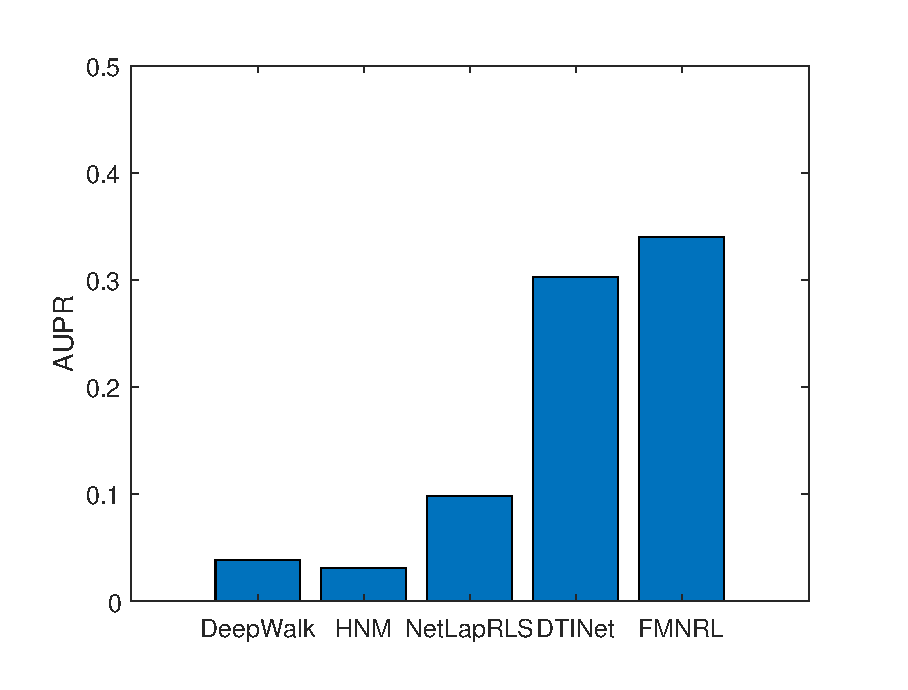
\includegraphics[width=5cm,height=3.5cm]{alldata_AUPR.eps}
\label{fig:allaupr}
}
\subfigure[AUROC]{
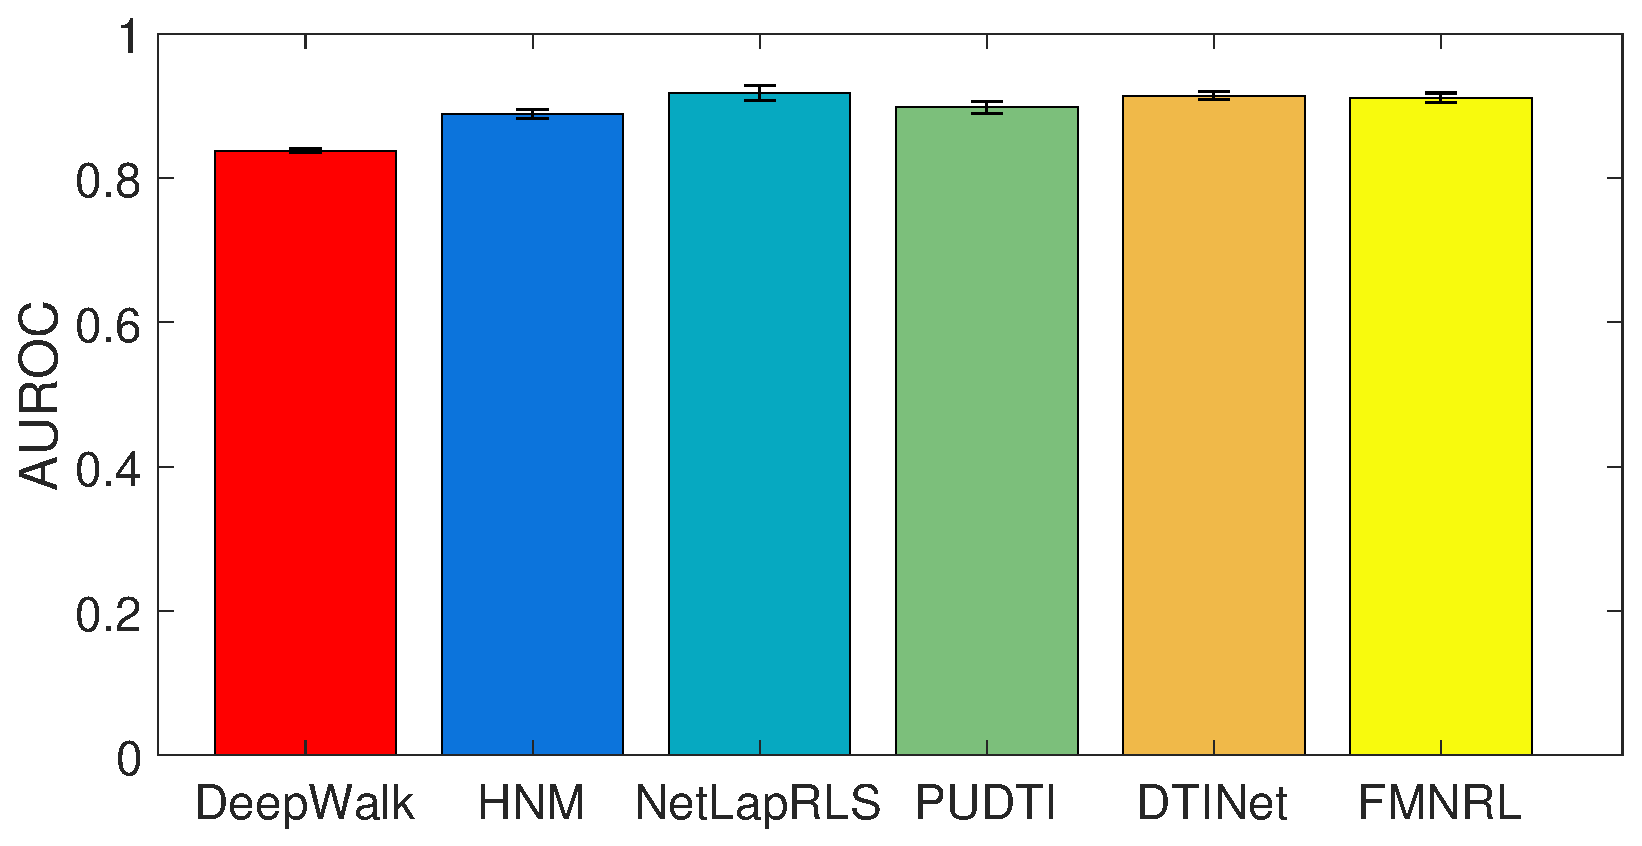
\includegraphics[width=5cm,height=3.5cm]{alldata_AUROC.eps}
\label{fig:allauroc}
}}
\vspace*{-10pt}
\caption{On the full dataset, FMNRL significantly boosts AUPR while obtaining comparable AUROC.}\label{fig:full}
\end{figure}

\begin{figure}[ht]
\centering
\scalebox{0.8}{
\subfigure[AUPR]{
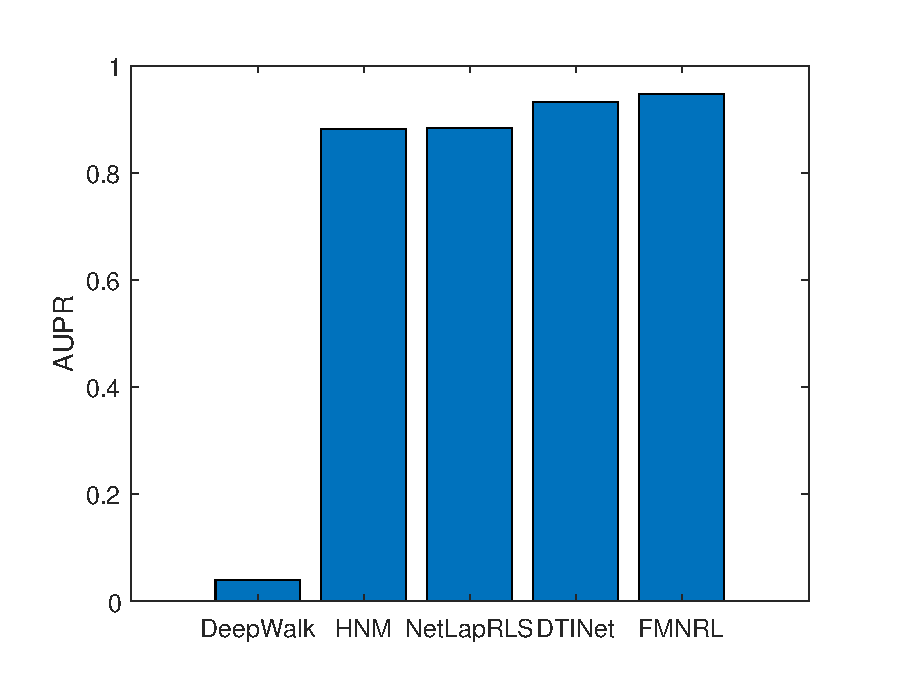
\includegraphics[width=5cm,height=3.5cm]{11data_AUPR.eps}
\label{fig:allaupr}
}
\subfigure[AUROC]{
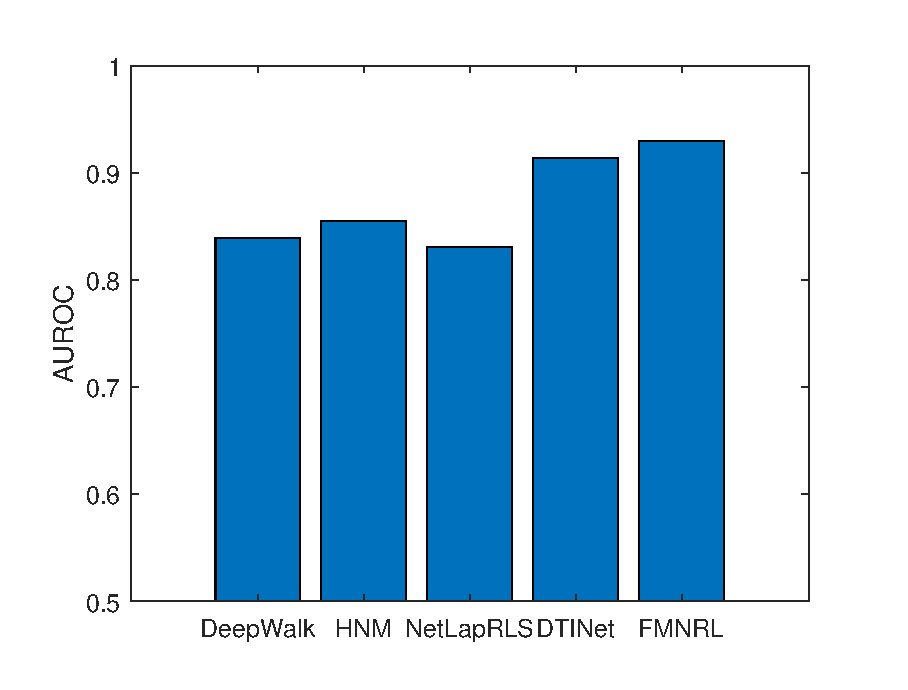
\includegraphics[width=5cm,height=3.5cm]{11data_AUROC.eps}
\label{fig:allauroc}
}}
\vspace*{-10pt}
\caption{On the sample dataset, FMNRL outperforms state-of-the-art methods in terms of both AUPR and AUROC.}\label{fig:sample}

\end{figure}

The comparative performance on the sample dataset are shown in Fig.~\ref{fig:sample}. We can see that (1) FMNRL model achieves better AUPR than all state-of-the-art methods. The best comparative method is DTINet, which achieves $93.20\%$. Our FMNRL model obtains a $94.66\%$ AUPR. (2) Most of the state-of-the-art methods have a higher AUPR result on the sample dataset than the full dataset, due to the balanced ratio of positive and negative samples. (3) Surprisingly DeepWalk has a very low AUPR performance on the sample set. (4) FMNRL model outperforms all state-of-the-art models in AUROC performance.  The best comparative method is again DTINet, which achieves $91.41\%$. Our FMNRL model obtains a $92.93\%$ AUROC. 

\textbf{Stability.} We next study the stability of our FMNRL model. We use various combination of $X$ and $Y$ as inputs. That is, we extract X from the four networks on the drug side (i.e. dd,di,de,ds) respectively, extract Y from the three networks on the protein side (i.e. pp, pd, ps) respectively, and use the $12$ combinations as inputs to train the model. The predictions are tested on the full dataset.

We compare the AUPR and AUROC performance of FMNRL and DTINet. As shown in Fig.~\ref{fig:stability}, FMNRL outperforms DTINet in most cases. FMNRL generates better AUPR results for $10$ feature combinations out of $12$. In term of AUROC, FMNR is better for $7$ feature combinations. The result shows that the performance improvement is stable. Change of feature representations does not affect FMNRL's ability to learn a better feature mapping space.

\begin{figure}[!ht]
\centering
\subfigure[AUPR]{
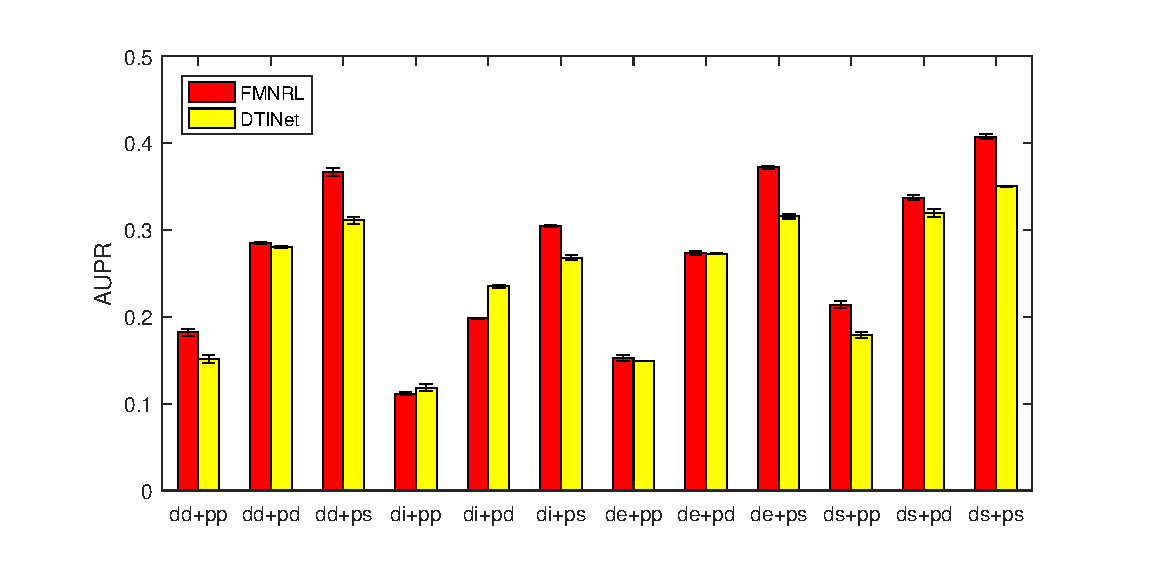
\includegraphics[width=8cm]{stability_AUPR.eps}
\vspace*{-5pt}
\label{fig:stabilityaupr}
}

\subfigure[AUROC]{
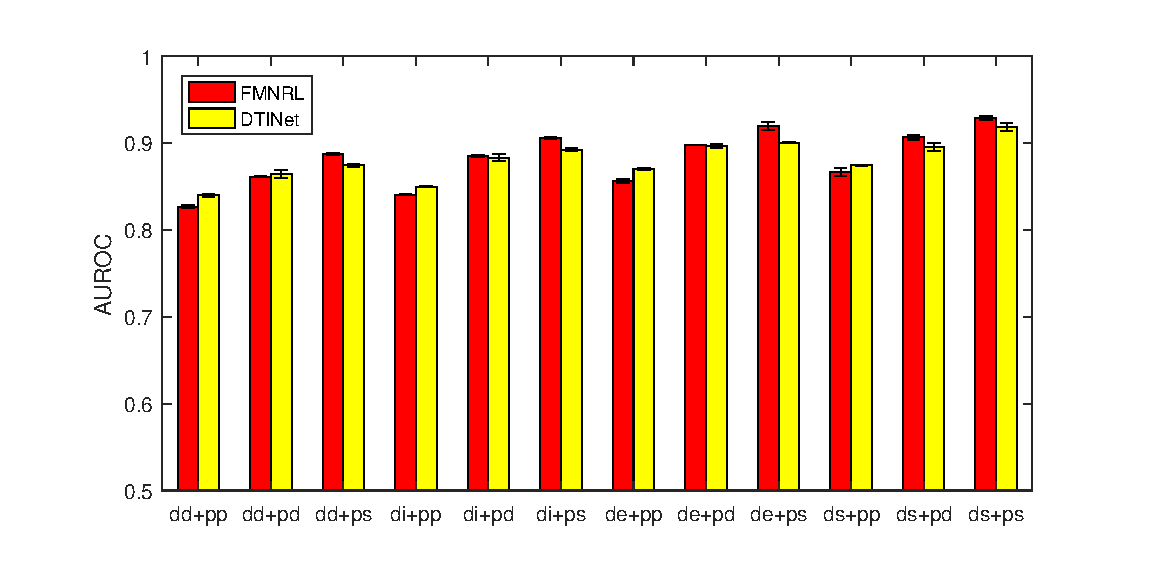
\includegraphics[width=8cm]{stability_AUROC.eps}
\label{fig:stabilityauroc}
}
\vspace*{-10pt}
\caption{Our model is stable with different feature inputs.}\label{fig:stability}
\end{figure}





\textbf{Parameter Tunning.} Finally we study the effects of parameters $K,L$. We first fix the parameter $L=400$ and tune the parameter $K=50,100,200,300,400,500$. We can see from Fig.~\ref{fig:k} and Fig.~\ref{fig:l} that the best number of drug features is around $100$, and the best number of target features is $400$. An appropriate number of drug features is important. When the number of drug features is too large, i.e. $K>200$, we observe a descent fall in both AUPR and AUROC. However, the model performance is less sensitive to the number of target features. For $L>500$, AUPR and AUROC remain the same.   

\begin{figure}[!ht]
\centering
\subfigure[$K$ number of drug features]{
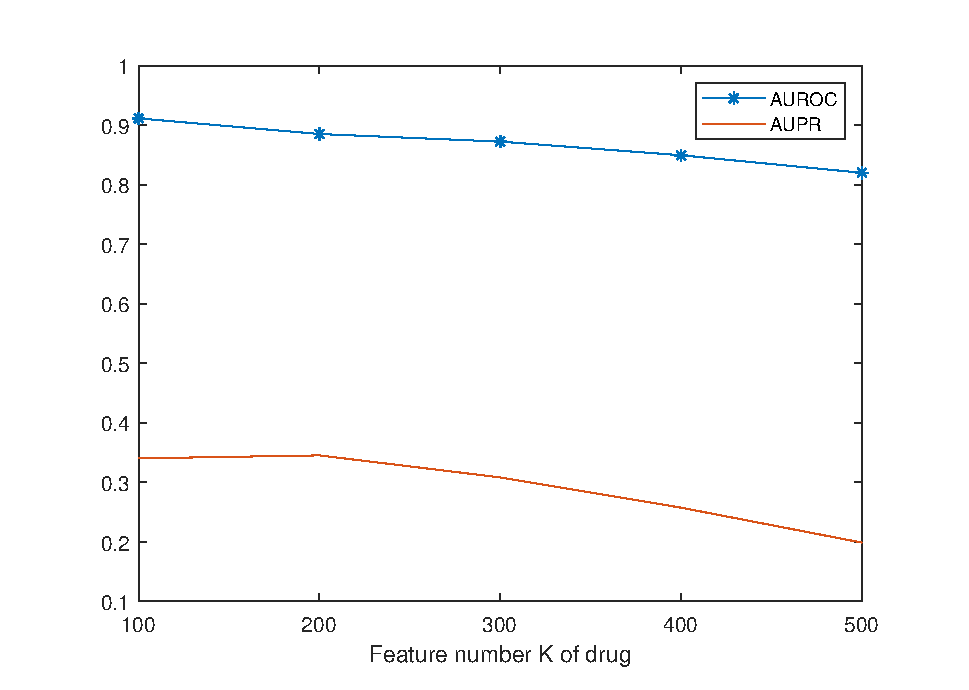
\includegraphics[width=4cm]{parameter_experiment_drug_feature.eps}
\label{fig:k}
}
\subfigure[$L$ number of protein features]{
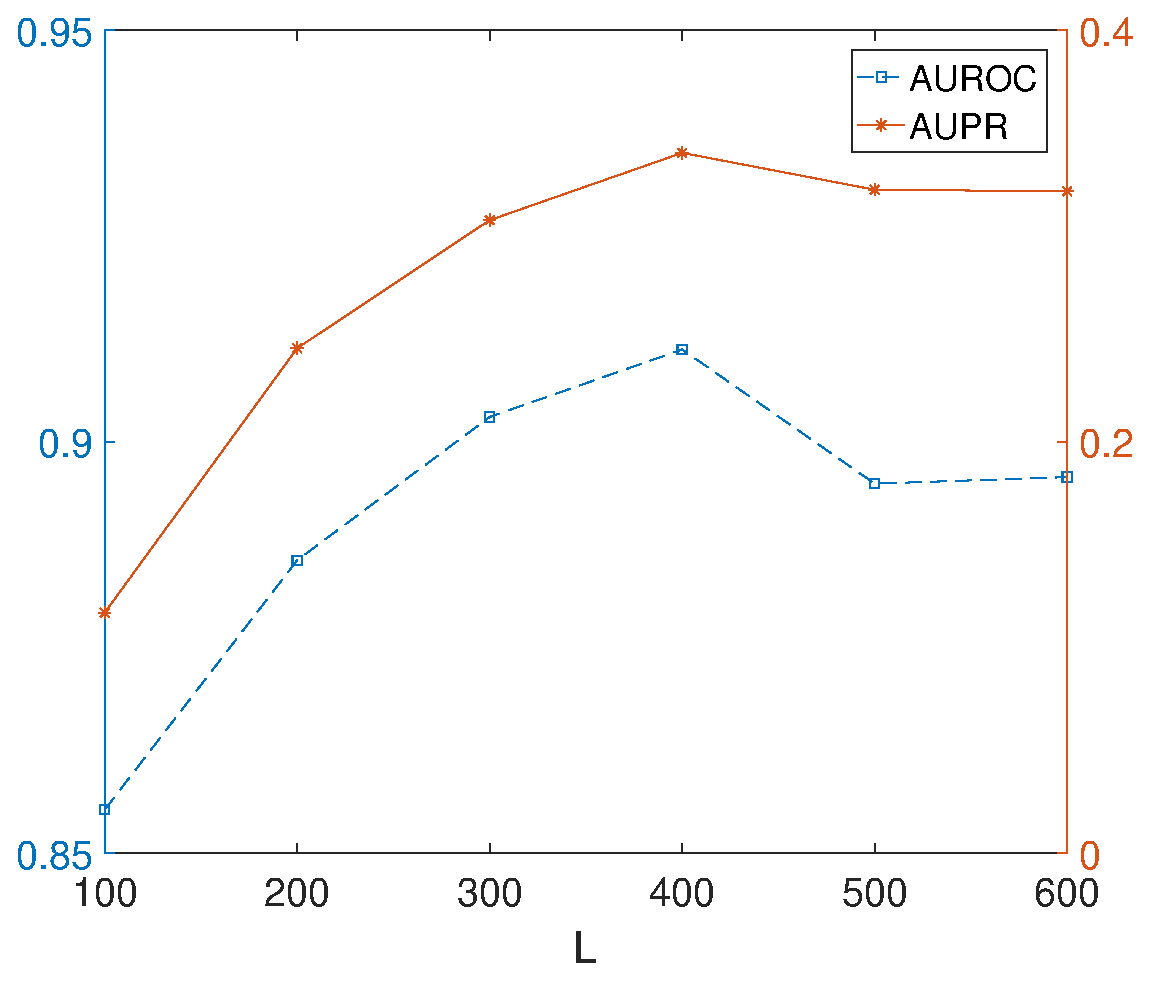
\includegraphics[width=4cm]{parameter_experiment_protein_feature.eps}
\label{fig:l}
}
\vspace*{-10pt}
\caption{AUPR and AUROC performance of our model with different number of drug and protein features.}\label{fig:parameter}
\end{figure}



\section{Conclusion}\label{sec:conclusion}

We propose a novel DTI prediction model based on the assumption that unknown DTI labels are missing not at random. By associating the status of a DTI being labelled or unknown to the sign of the DTI label, our proposed FMNRL model can learn a better feature mapping from drug feature space to target feature space. We experimentally demonstrate that FMNRL outperforms state-of-the-art computational DTI identification methods. This work sheds some insights into fully exploiting the information in unknown DTIs. Our further directions include improving the factorization framework and analyzing the missing mechanisms. 

\begin{thebibliography}{10}
\bibitem{Ding2013Similarity}
Ding, H., Takigawa, I., Mamitsuka, H., and Zhu, S.
\newblock Similarity-based machine learning methods for predicting drug–target interactions: a brief review. \newblock In {\em Briefings in bioinformatics}, 15(5), 734-747.
\bibitem{Peng2017Screening}
Peng L, Zhu W, Liao B, et al.
\newblock Screening drug-target interactions with positive-unlabeled learning.
\newblock In {\em Scientific Reports}, 2017, 7(1): 8087.

\bibitem{Little1987Statistical}
R. J. A. Little and D. B. Rubin.
\newblock Statistical Analysis with Missing Data, 1987.

\bibitem{Luo2017Network}
Luo Y, Zhao X, Zhou J, et al.
\newblock A network integration approach for drug-target interaction prediction and computational drug repositioning from heterogeneous information.
\newblock In {\em Nature Communications}, 2017, 8(1).

\bibitem{Xia2010Semi}
Xia Z, Wu L Y, Zhou X, et al. 
\newblock Semi-supervised drug-protein interaction prediction from heterogeneous biological spaces. 
\newblock In {\em Bmc Systems Biology}, 2010, 4(S2):1-16.

\bibitem{Wang2014Drug}
Wang W, Yang S, Zhang X, et al. 
\newblock Drug repositioning by integrating target information through a heterogeneous network model. 
\newblock In {\em Bioinformatics}, 2014, 30(20):2923-2930.

\bibitem{Zong2017Deep}
Zong N, Kim H, Ngo V, et al. 
\newblock Deep Mining Heterogeneous Networks of Biomedical Linked Data to Predict Novel Drug-Target Associations. 
\newblock In {\em Bioinformatics}, 2017, 33(15).

%\bibitem{DrugBank}
%Knox, C. et al. Drugbank 3.0: a comprehensive resource for 'omics' research on drugs. Nucleic Acids Res. 39, D1035-D1041 (2011).
%
%\bibitem{ProteinDatabase}
%Prasad, T. S. K. et al. Human protein reference database-2009 update. Nucleic Acids Res. 37, D767-D772 (2009).
%
%\bibitem{ToxicogenomicsDatabase}
%Davis, A. P. et al. The comparative toxicogenomics database: update 2013. Nucleic Acids Res. 41, D1104-D1114 (2013).
%
%\bibitem{SideEffect}
%Kuhn, M., Campillos, M., Letunic, I., Jensen, L. J. and  Bork, P. A side effect resource to capture phenotypic effects of drugs. 6, 343 (2009).
\end{thebibliography}
%\balancecolumns
\end{document}